\documentclass[12pt]{article}
\setlength{\oddsidemargin}{0in}
\setlength{\evensidemargin}{0in}
\setlength{\textwidth}{6.5in}
\setlength{\parindent}{0in}
\setlength{\parskip}{\baselineskip}

\usepackage{amsmath,amsfonts,amssymb,fancyvrb,tikz}
\usetikzlibrary{matrix,calc,circuits.logic.US,shapes}
\tikzset{>=latex}
\usepackage{graphicx}
\usepackage{fancyhdr}
\usepackage[margin=1in]{geometry}
\pagestyle{fancy}

\addtolength{\topmargin}{30pt}
\setlength{\textheight}{8in}


\begin{document}

\rhead{{\bf CSCI 3104 \\Problem Set 4\\ Spring 2017, CU-Boulder}}
\lhead{{\bf 
        Sam Cuthbertson (06/16)\\ 
        Grant Baker (07/23) \\ 
        Connor Hudson (05/07)}}
\renewcommand{\headrulewidth}{0.4pt}
\headheight = 43pt

\vspace{-3mm}

\begin{enumerate}
	% question 1
	\item (10 pts) \textit{Given the red-black trees $T_{1}$ and $T_{2}$, which contain $m$ and $n$ elements respectively, we want to determine whether they have some particular key in common. Assume an adversarial sequence 
that placed the $m$ and $n$ items into the two trees.}

	\begin{enumerate}

	\item \textit{Suppose our algorithm traverses each node of $T_{1}$ using an in-order traversal and checks if the key corresponding to the current node traversed exists in $T_{2}$. Express the asymptotic running time of this 
procedure, in terms of $m$ and $n$.}
	
	There are $m$ elements in $T_1$. An in-order traversal of $T_1$ will therefore take $O(m)$, since we are visiting each element exactly once.
	
	For each element in $T_1$, we search $T_2$ for its key. The maximum height of $T_2$ is $2\log_2(n+1)$, and since it is organized by key, searching will therefore take $O(\log_2 n)$. We perform this search for each element 
in $T_1$, or $m$ times total.
	
	So the asymptotic running time of this algorithm is
	\[
	\boxed{T(m,n) = m\left(2\log_2(n+1)\right) = O(m\log_2 n)}
	\]

	\item \label{q:rb:hash:b} \textit{Now suppose our algorithm first allocates a new hash table $H_{1}$ of size $m$ (assume $H_{1}$ uses a uniform hash function) and then inserts every key in $T_{1}$ into $H_{1}$ during a 
traversal of $T_{1}$. Then, we traverse the tree $T_{2}$ and search for whether the key of each node traversed already exists in $H_{1}$. Give the asymptotic running time of this algorithm in the average case. Justify your answer.}
	
	The running time for the allocation of the hash table is $O(m)$, and uniform insertion of each key of $T_1$ is $O(m)$, since that is the running time of a traversal of $T_1$.
	
	Then, the traversal of the tree $T_2$ takes $O(n)$. Searching for the key on each node of the traversal is $O(1)$ due to the assumption of a uniform hash function.
	
	Therefore, the total runtime of this algorithm is the sum of the two tree traversals, or 
	\[
	\boxed{T(m,n) = O(m+n)}
	\]
	
	% \textsf{I'll do this one -G}

	\end{enumerate}


    % question 2
    \newpage
	\item (30 pts) \textit{Voldemort is writing a secret message to his lieutenants and wants to prevent it from being understood by mere Muggles. He decides to use Huffman encoding to encode the message. Magically, the symbol 
frequencies of the message are given by the \textit{Lucas numbers}, a famous sequence of integers discovered by the same person who discovered the \textit{Fibonacci numbers}. The $n$th Lucas number is defined as $L_{n} = 
L_{n-1}+L_{n-2}$ for $n>1$ with base cases $L_{0}=2$ and $L_{1}=1$.}

	\begin{enumerate}

	\item \label{q:huff:a} \textit{For an alphabet of $\Sigma=\{a,b,c,d,e,f,g,h\}$ with frequencies given by the first $|\Sigma|$ Lucas numbers, give an optimal Huffman code and the corresponding encoding tree for Voldemort to 
use.}
	
	% "In 1951, David A. Huffman and his MIT information theory classmates were given the choice of a term paper or a final exam. The professor, Robert M. Fano, assigned a term paper on the problem of finding the most efficient 
binary code. Huffman, unable to prove any codes were the most efficient, was about to give up and start studying for the final when he hit upon the idea of using a frequency-sorted binary tree and quickly proved this method the 
most efficient." LEGENDARY
	
	The first 8 Lucas numbers are $2, 1, 3, 4, 7, 11, 18, 29$ so our frequency table is $\{b: 1, a: 2, c: 3, d: 4, e: 7, f: 11, g: 18, h: 29\}$. After applying Huffman's algorithm, we get the following encoding tree/code: 
	
	%Hey look, a tree!
	\begin{center}
	\resizebox{.7\textwidth}{!}{%
		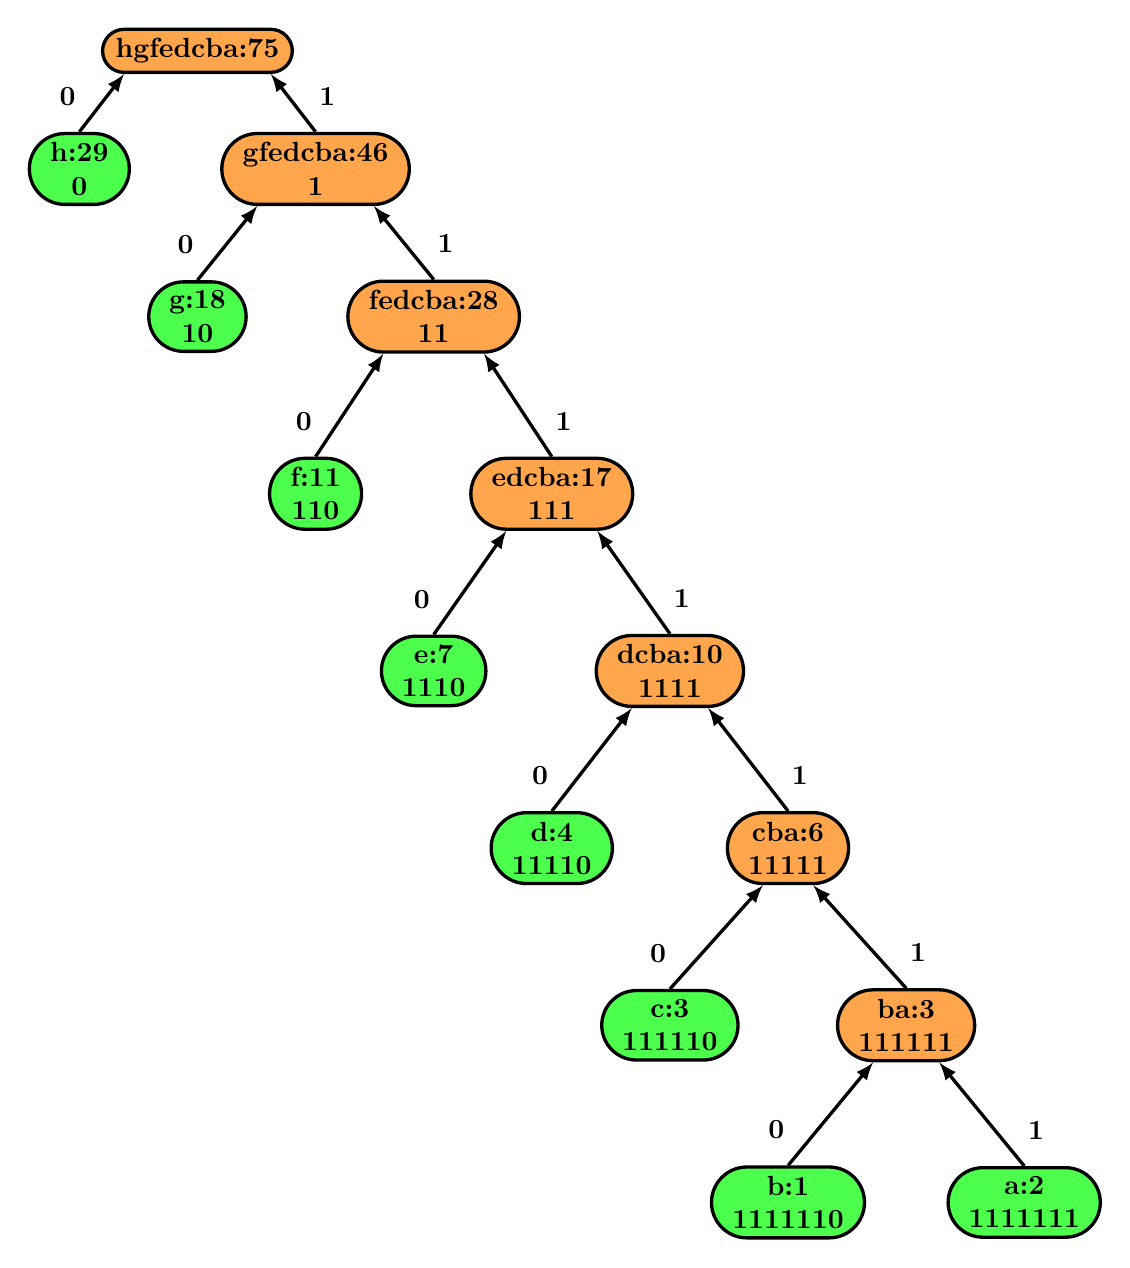
\begin{tikzpicture}[circuit logic US,scale=1.5]
			\node[rounded rectangle, very thick, draw=black, fill=orange!70] (hgfedcba) at (3,3) {\textbf{hgfedcba:75}};
			
			\node[rounded rectangle, very thick, draw=black, fill=green!70, align=center] (h) at (2,2) { \textbf{h:29} \\ \textbf{0}};
			\node at ($(h.north) + (-0.1,0.3)$) {\textbf{0}};
            \draw [->,very thick] (h.north) -- (hgfedcba.south west);
            
            \node[rounded rectangle, very thick, draw=black, fill=orange!70, align=center] (gfedcba) at (4,2) {\textbf{gfedcba:46} \\ \textbf{1}};
			\node at ($(gfedcba.north) + (0.1,0.3)$) {\textbf{1}};
            \draw [->,very thick] (gfedcba.north) -- (hgfedcba.south east);
            
            \node[rounded rectangle, very thick, draw=black, fill=green!70, align=center] (g) at (3,0.75) {\textbf{g:18} \\ \textbf{10}};
			\node at ($(g.north) + (-0.1,0.3)$) {\textbf{0}};
            \draw [->,very thick] (g.north) -- (gfedcba.south west);
            
            \node[rounded rectangle, very thick, draw=black, fill=orange!70, align=center] (fedcba) at (5,0.75) {\textbf{fedcba:28} \\ \textbf{11}};
			\node at ($(fedcba.north) + (0.1,0.3)$) {\textbf{1}};
            \draw [->,very thick] (fedcba.north) -- (gfedcba.south east);
            
            \node[rounded rectangle, very thick, draw=black, fill=green!70, align=center] (f) at (4,-.75) {\textbf{f:11} \\ \textbf{110}};
			\node at ($(f.north) + (-0.1,0.3)$) {\textbf{0}};
            \draw [->,very thick] (f.north) -- (fedcba.south west);
            
            \node[rounded rectangle, very thick, draw=black, fill=orange!70, align=center] (edcba) at (6,-.75) {\textbf{edcba:17} \\ \textbf{111}};
			\node at ($(edcba.north) + (0.1,0.3)$) {\textbf{1}};
            \draw [->,very thick] (edcba.north) -- (fedcba.south east);
            
            \node[rounded rectangle, very thick, draw=black, fill=green!70, align=center] (e) at (5,-2.25) {\textbf{e:7} \\ \textbf{1110}};
			\node at ($(e.north) + (-0.1,0.3)$) {\textbf{0}};
            \draw [->,very thick] (e.north) -- (edcba.south west);
            
            \node[rounded rectangle, very thick, draw=black, fill=orange!70, align=center] (dcba) at (7,-2.25) {\textbf{dcba:10} \\ \textbf{1111}};
			\node at ($(dcba.north) + (0.1,0.3)$) {\textbf{1}};
            \draw [->,very thick] (dcba.north) -- (edcba.south east);
            
            \node[rounded rectangle, very thick, draw=black, fill=green!70, align=center] (d) at (6,-3.75) {\textbf{d:4} \\ \textbf{11110}};
			\node at ($(d.north) + (-0.1,0.3)$) {\textbf{0}};
            \draw [->,very thick] (d.north) -- (dcba.south west);
            
            \node[rounded rectangle, very thick, draw=black, fill=orange!70, align=center] (cba) at (8,-3.75) {\textbf{cba:6} \\ \textbf{11111}};
			\node at ($(cba.north) + (0.1,0.3)$) {\textbf{1}};
            \draw [->,very thick] (cba.north) -- (dcba.south east);
    
            \node[rounded rectangle, very thick, draw=black, fill=green!70, align=center] (c) at (7,-5.25) {\textbf{c:3} \\ \textbf{111110}};
			\node at ($(c.north) + (-0.1,0.3)$) {\textbf{0}};
            \draw [->,very thick] (c.north) -- (cba.south west);
            
            \node[rounded rectangle, very thick, draw=black, fill=orange!70, align=center] (ba) at (9,-5.25) {\textbf{ba:3} \\ \textbf{111111}};
			\node at ($(ba.north) + (0.1,0.3)$) {\textbf{1}};
            \draw [->,very thick] (ba.north) -- (cba.south east);
            
            \node[rounded rectangle, very thick, draw=black, fill=green!70, align=center] (b) at (8,-6.75) {\textbf{b:1} \\ \textbf{1111110}};
			\node at ($(b.north) + (-0.1,0.3)$) {\textbf{0}};
            \draw [->,very thick] (b.north) -- (ba.south west);
            
            \node[rounded rectangle, very thick, draw=black, fill=green!70, align=center] (a) at (10,-6.75) {\textbf{a:2} \\ \textbf{1111111}};
			\node at ($(a.north) + (0.1,0.3)$) {\textbf{1}};
            \draw [->,very thick] (a.north) -- (ba.south east);
		\end{tikzpicture}
	}
	\end{center}
	\[
	\boxed{\{a: 1111111,\ b: 1111110,\ c: 111110,\ d: 11110,\ e: 1110,\ f: 110,\ g: 10,\ h: 0\}}
	\]

	\item \textit{Recall that in the Huffman algorithm, we may specify a simple convention that determines the way a pair of dequeued symbols are arranged in the coding tree relative to their parent. How many optimal Huffman 
codes could you have provided to Voldemort for the set of frequencies in part (\ref{q:huff:a})? Justify your answer.} 
	
	Note that we can easily create a different optimal tree by breaking the tie at the bottom of the tree differently. For example, we choose the `@c' node to be the left leaf, when we also could have chosen to set it as the 
right leaf. Similarly, we could set the convention that right children are 0 and left children are 1, which would yield a different tree, and there would be two possible trees for that convention due to the `c/bc' tie. That means 
there are \textbf{four possible optimal code trees} for the given symbols. \\

	\item \textit{Generalize your answer to (\ref{q:huff:a}) and give the structure of an optimal code when the frequencies are the first $n$ Lucas numbers.}
	
	We note that the Lucas numbers are always increasing at such a rate that a generalized encoding tree for an alphabet of $n$ symbols where the frequencies are the first $n$ Lucas numbers is given by:
	
	\begin{center}
	\resizebox{.85\textwidth}{!}{%
		\begin{tikzpicture}[circuit logic US,scale=1.5]
			\node[rounded rectangle, very thick, draw=black, fill=orange!70] (1...n) at (3,3) {\textbf{1...n:Lucas(n + 3) - 1}};
			
			\node[rounded rectangle, very thick, draw=black, fill=green!70, align=center] (n) at (1.5,1.5) { \textbf{n:Lucas(n)} \\ \textbf{0}};
			\node at ($(n.north) + (-0.1,0.3)$) {\textbf{0}};
            \draw [->,very thick] (n.north) -- (hgfedcba.south west);
            
            \node[rounded rectangle, very thick, draw=black, fill=orange!70, align=center] (gfedcba) at (4.5,1.5) {\textbf{1..(n-1):Lucas(n+2)} \\ \textbf{1}};
			\node at ($(gfedcba.north) + (0.1,0.3)$) {\textbf{1}};
            \draw [->,very thick] (gfedcba.north) -- (hgfedcba.south east);
            
            \node[rounded rectangle, very thick, draw=black, fill=green!70, align=center] (g) at (3,0) {\textbf{(n-1):Lucas(n-1)} \\ \textbf{10}};
			\node at ($(g.north) + (-0.1,0.3)$) {\textbf{0}};
            \draw [->,very thick] (g.north) -- (gfedcba.south west);
            
            \node[rounded rectangle, very thick, draw=black, fill=orange!70, align=center] (edcba) at (7.5,-1.25) {\textbf{1,2:Lucas(3)} \\ \textbf{111111... (n-2 times)}};
			\node at ($(edcba.north) + (0.1,0.3)$) {\textbf{1}};
            \draw [->,very thick,dashed] (edcba.north) -- (gfedcba.south east);
            
            \node[rounded rectangle, very thick, draw=black, fill=green!70, align=center] (e) at (5.5,-2.75) {\textbf{2:1} \\ \textbf{11111... (n-2 times)0}};
			\node at ($(e.north) + (-0.1,0.3)$) {\textbf{0}};
            \draw [->,very thick] (e.north) -- (edcba.south west);
            
            \node[rounded rectangle, very thick, draw=black, fill=green!70, align=center] (dcba) at (9.25,-2.75) {\textbf{1:2} \\ \textbf{11111... (n-1 times)}};
			\node at ($(dcba.north) + (0.1,0.3)$) {\textbf{1}};
            \draw [->,very thick] (dcba.north) -- (edcba.south east);
            

		\end{tikzpicture}
	}
	\end{center}

	\end{enumerate}


    % question 3
    % See https://mitpress.mit.edu/sicp/full-text/book/book-Z-H-11.html#%_idx_728
    \newpage
	\item (30 pts total) \textit{Draco Malfoy is struggling with the problem of making change for $n$ cents using the smallest number of coins. Malfoy has coin values of $v_{1}>v_{2}>\dots>v_{r}$ for $r$ coins types, where each 
coin's value $v_{i}$ is a positive integer, and where $v_{1}$ is the most valuable coin. His goal is to obtain a set of counts $\{d_{i}\}$, one for each coin type, such that $\sum_{i=1}^{r}d_{i}=k$ and where $k$ is minimized.}

	\begin{enumerate}

	\item \textit{A greedy algorithm for making change is the \textbf{cashier's algorithm}, which all young wizards learn. Malfoy writes the following pseudocode on the whiteboard to illustrate it, where $n$ is the amount of 
money to make change for and $v$ is a vector of the coin denominations:}
	\begin{small}
	\begin{verbatim}
	0| wizardChange(n,v):
	1|    d[1 .. v.len()] = 0  // initial histogram of coin types in solution
	2|    while n > 0 {
	3|       k = r
	4|       while ( v[k] > n and k >= 0 ) { k-- }
	5|       if k==0 { return 'no solution' }
	6|       else { d[k]++ }
	7|    }
	8|    return d
	\end{verbatim}
	\end{small}
	\textit{Hermione snorts and says Malfoy's code has bugs. Identify the bugs and explain why each would cause the algorithm to fail.}
	
    \begin{itemize}
        \item On line 3, $\texttt{k=r}$ should be $\texttt{k=1}$ as the largest coin value will be in position 1, and $\texttt{r}$ is undefined.
        \item On line 4, $\texttt{k--}$ should be $\texttt{k++}$ as the algorithm begins by first checking the largest item, not the smallest item. Additionally, $\texttt{k>=0}$ should be $\texttt{k<=v.len()+1}$ as the loop should 
break when we have no currency small enough.
        \item On line 5, $\texttt{k==0}$ should be $\texttt{k==v.len()+1}$ as the algorithm will fail when it runs out of coins of small enough values.
    \end{itemize}
    
	\item \textit{Sometimes the goblins at Gringotts Wizarding Bank run out of coins, and make change using whatever is left on hand. Identify a set of U.S. coin denominations for which the greedy algorithm does not yield an 
optimal solution. Justify your answer in terms of optimal substructure and the greedy-choice property. (The set should include a penny so that there is a solution for every value of $n$.)\footnote{Assistance from Matt Maierhofer}}

	Consider the set of $\{1,10,25\}$ coins for $30c$. The greedy algorithm would choose $\{25, 1, 1, 1, 1, 1\}$ as 25 is the greedy-choice first step, while the optimal choice is clearly $\{10,10,10\}$. As the optimal first 
choice (10) is not equal to the greedy first choice (25), there is no guaranteed optimal substructure for the given set of coins. \\
	
	\item \textit{On the advice of computer scientists, Gringotts has announced that they will be changing all wizard coin denominations into a new set of coins denominated in powers of $c$, i.e., denominations of $c^{0}, 
c^{1}, \dots , c^{\ell}$ for some integers $c>1$ and $\ell\geq 1$. (This will be done by a spell that will magically transmute old coins into new coins, before your very eyes.) Prove that the cashier's algorithm will always yield 
an optimal solution in this case.}

	\textit{Hint: consider the special case of $c=2$.}\\
	
% 	\textsf{This proof is easy, and I'll do it -G}
	
	Consider an amount of money, and denote this amount $n_{\ell}$. Let our set of coin denominations be $c^0,...,c^{\ell}$. We shall consider a truncated base-$c$ expansion of $n$.
	
	We have also a set of counts $d_0,...,d_{\ell}$ such that 
	\[
	n_{\ell} = \sum_{i=0}^{\ell} d_i c^i
	\]
	If we examine the cashier's algorithm, at the first step it finds the largest number of the largest denomination of coin less than $n_{\ell}$. In other words, it finds an integers $d_{\ell}$ such that 
	\[
	n_{\ell} = d_{\ell} c^{\ell} + n_{\ell-1}
	\]
	where $n_{\ell-1}$ is nonnegative. Here, $d_{\ell}$ may be any nonnegative integer.
	Then, on the next step it computes a $d_{\ell-1}$ in a similar fashion
	\[
	n_{\ell-1} = d_{\ell-1} c^{\ell-1} + n_{\ell-2}
	\]
	In general, on the $k$-th step, the algorithm has an amount $n_{\ell-k+1}$ and it wishes to compute $d_{\ell-k+1}$ such that 
	\[
	n_{\ell-k+1} = d_{\ell-k+1} c^{\ell-k+1} + n_{\ell-k}
	\]
	The existence of $d_{\ell-k+1}$ and $n_{\ell-k}$ is guaranteed by Euclidian division.
	
	We also have that $\forall k \in \{0,...,\ell-1\}$, $d_k \in \{0,...,c-1\}$. This is because if $d_k = \alpha \geq c$, then on the previous step the Euclidian division was erroneous because $d_{k+1}$ is computed such that 
$n_k\in\{0,...,c^k-1\}$.
	
	Further, this is exactly the computation of the truncated base-$c$ expansion of $n_{\ell}$. The only difference is in $d_{\ell}$, whose value can be any nonnegative integer rather than just in the set $\{0,...,c-1\}$.
	
	Therefore, the cashier's algorithm produces the truncated base-$c$ expansion of $n_{\ell}$.
	
	This is the optimal solution. We will show this by contradiction.
	
	First, have $\{d_0,...,d_{\ell}\}$ as the computed truncated base-$c$ expansion of $n_{\ell}$. Assume that there is a more optimal set $\{\delta_0,...,\delta_{\ell}\}$.
	
	Then, we have that 
	\[
	\sum_{i=0}^{\ell} d_i -\sum_{i=0}^{\ell} \delta_i > 0
	\]
	By shifting terms, we have that
	\[
	\sum_{i=0}^{\ell} d_i - \delta_i > 0
	\]
	This means that $\exists i\in\{0,...,\ell\}$ such that $d_i\neq \delta_i$.
	But, we know that 
	\[
	n_{\ell} = \sum_{i=0}^{\ell} d_i c^i = \sum_{i=0}^{\ell} \delta_i c^i
	\]
	Computing $n_{\ell-1}$ from each sum, we have that 
	\[
	n_{\ell-1} = \sum_{i=0}^{\ell-1} d_i c^i = \sum_{i=0}^{\ell-1} \delta_i c^i
    \]
    where $d_i$ and $\delta_i$ are $\{0,...,c-1\}$.
    
    This implies that there are two distinct base-$c$ expansions for $n_{\ell-1}$. However, base-$c$ expansions are always unique for $c>1$. This is a contradiction.\\
    
    Therefore, the cashier's algorithm using the denominations $c^0,...,c^{\ell}$ will always produce the truncated base-$c$ expansion of the amount, and that the truncated base-$c$ expansion is always the optimal solution.
    
	\end{enumerate}


    % question 4
    \newpage
	\item (30 pts) \textit{Consider the following hash function. Let $U$ be the universe of strings composed of the characters from the alphabet $\Sigma=[${\tt A}$,\dots,${\tt Z}$]$, and let the function $f(x_{i})$ return the 
index of a letter $x_{i}\in \Sigma$, e.g., $f(${\tt A}$)=1$ and $f(${\tt Z}$)=26$. Finally, for an $m$-character string $x\in \Sigma^{m}$, define $h(x) = \left(\left[\sum_{i=1}^{m}f(x_{i})\right]\!\! \mod \ell\right)$, where $\ell$ 
is the number of buckets in the hash table. That is, our hash function sums up the index values of the characters of a string $x$ and maps that value onto one of the $\ell$ buckets.}

	\begin{enumerate}

	\item \textit{The following list contains US Census derived last names: \\
	{\tt http://www2.census.gov/topics/genealogy/1990surnames/dist.all.last} \\
	Using these names as input strings, first choose a uniformly random 50\% of these name strings and then hash them using $h(x)$. Produce a histogram showing the corresponding distribution of hash locations when $\ell=200$. 
Label the axes of your figure. Brief description what the figure shows about $h(x)$; justify your results in terms of the behavior of $h(x)$. Do not forget to append your code.\footnote{Invaluable assistance from {\tt 
http://reference.wolfram.com/language/}}}
	
	\begin{center}
	    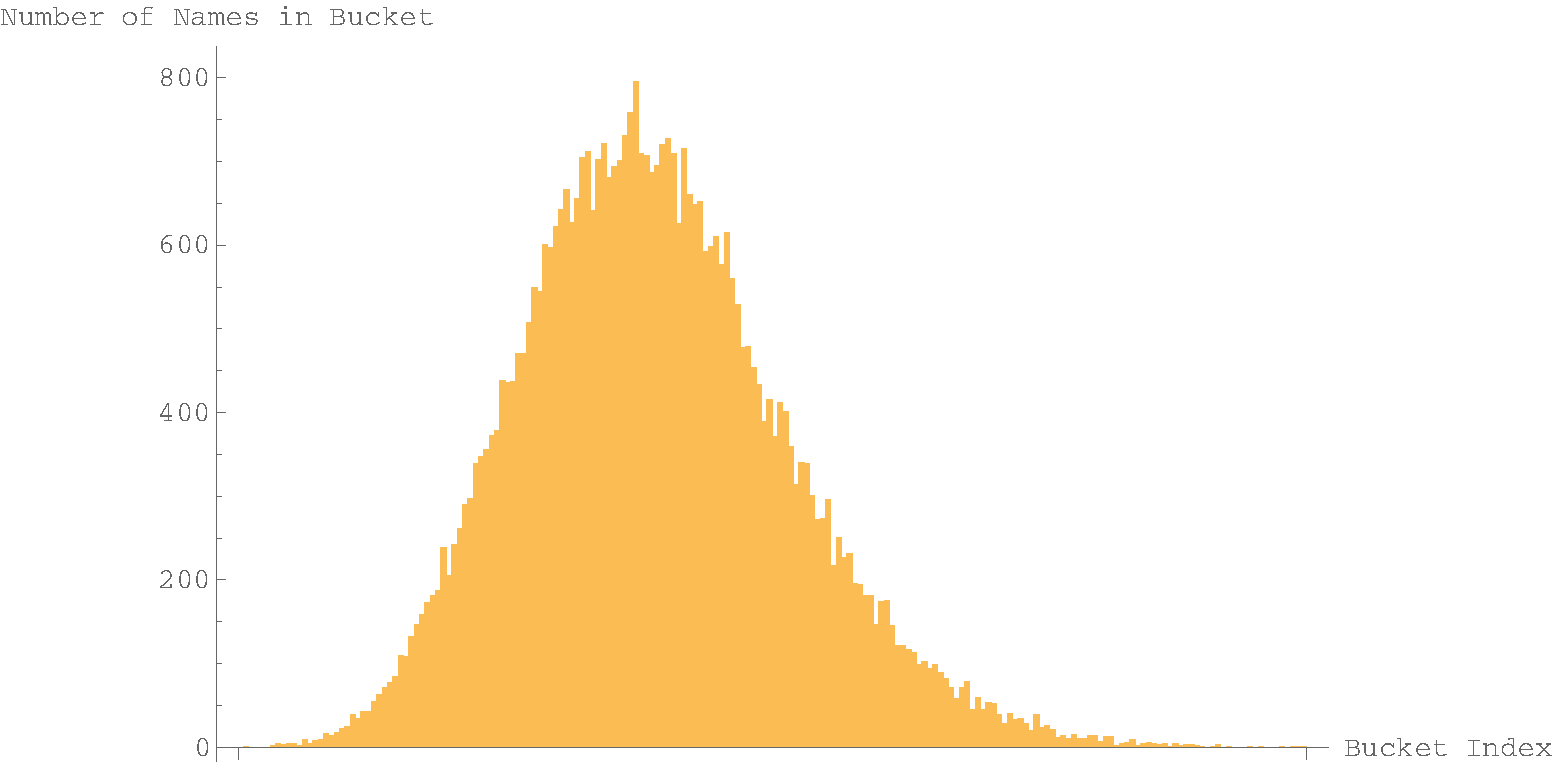
\includegraphics[width=.8\textwidth]{4a}
    \end{center}
    The above figure displays the distribution of outputs from $h(x)$. We can see that most names are being hashed to the same range of indexes, roughly between 50 and 150. That make sense in relation to $h(x)$, as it simply sums 
up the value of the input name's letters, and most last names in America tend to be of similar lengths. 
	\\
	\item \textit{Enumerate at least 4 reasons why $h(x)$ is a bad hash function relative to the ideal behavior of uniform hashing.}
	
	\begin{itemize}
	    \item We note that items tend to get hashed in a select few buckets near the middle.
	    \item Many of the buckets on either end, especially buckets $>160$, are empty.
	    \item Out of the buckets that are filled, some are filled much more than others (In the range of 8 to 800 elements).
	    \item $h(x)$ here seems to reveal something about the data, showing a Gaussian distribution. A uniform hashing function would reveal nothing about the input data, instead sorting uniformly regardless of any innate 
properties of the input.
	\end{itemize}

	\item (10 pts extra credit) \textit{Produce a plot showing how the length of the longest chain (were we to use chaining for resolving collisions) grows as a function of the number $n$ of these strings that we hash into a 
table with $\ell=200$ buckets. Comment on this trend using the language of the asymptotic growth of functions, worst-case scenarios, and loading factors of hash tables.}
	
	\begin{center}
	    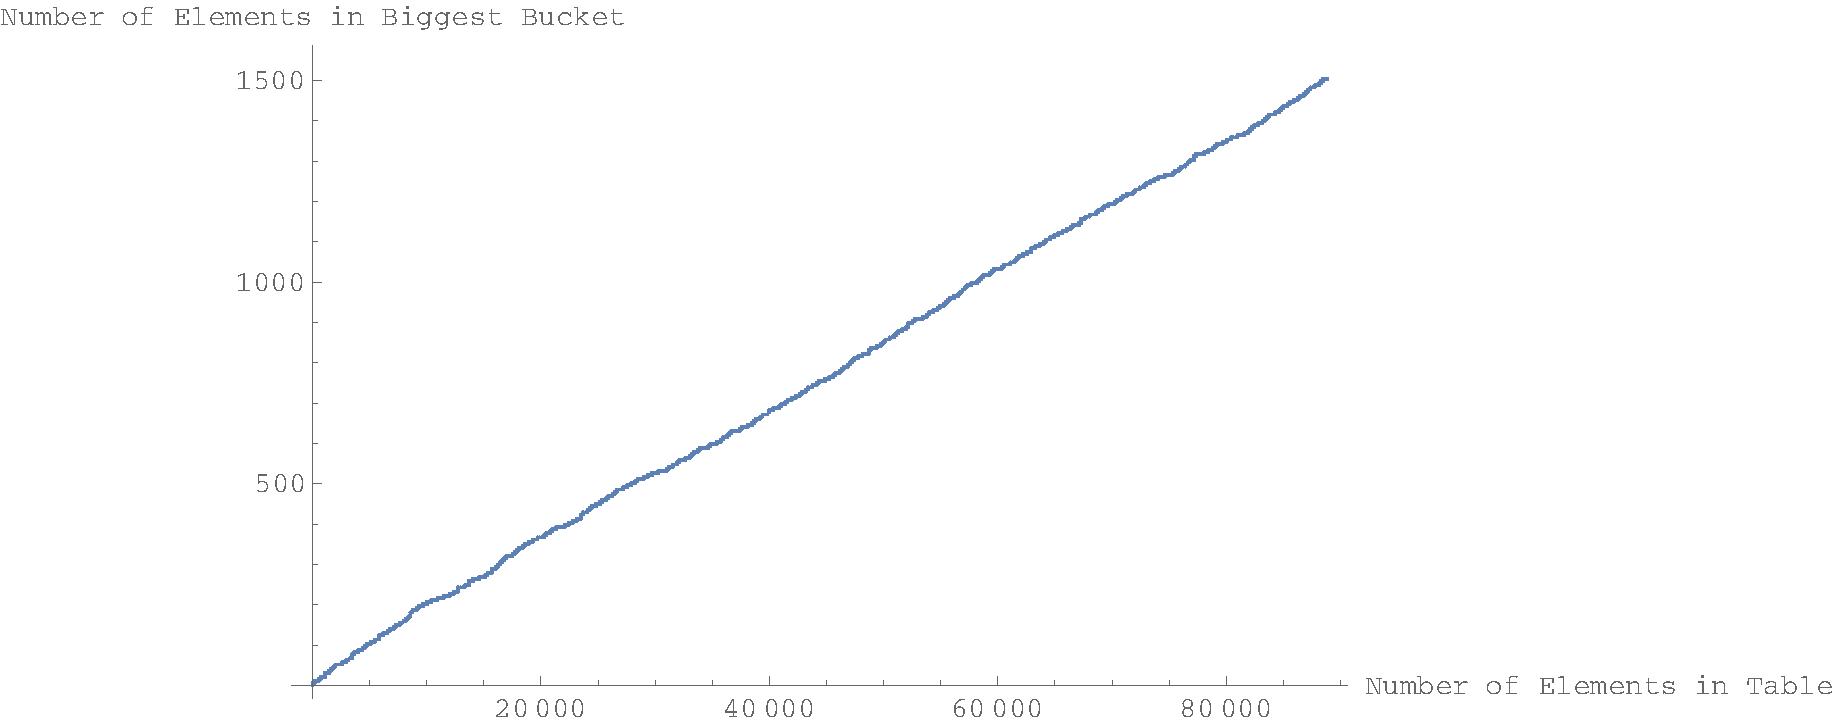
\includegraphics[width=.8\textwidth]{4c}
    \end{center}
    It appears that our longest chain grows linearly, on the order of $O(n)$. It's interesting to note that even when $\ell=20$ and $h(x)$ is decently uniform, this graph is still linear. Thus, even in either worst case scenario 
(poor hashing function, heavily loaded table), the growth of the largest chain will be $O(1)$. Additionally, this graph changes only in scale when the loading factor of the table is changed, meaning that the asymptotic growth of 
the longest chain is independent of loading factor. 
    
	\end{enumerate}
	
    % question 5
    \newpage
	\item (20 pts extra credit) \textit{Let $A$ and $B$ be arrays of integers. Each array contains $n$ elements, and each array is in sorted order (ascending). $A$ and $B$ do not share any elements in common. Give a $O(\lg 
n)$-time algorithm which finds the median of $A\, \cup\, B$ and prove that it is correct. This algorithm will thus find the median of the $2n$ elements that would result from putting $A$ and $B$ together into one array. (Note: 
define the median to be the average of the two middle values of a list with an even number of elements.)}\footnote{Properties of the median from Miller and Miller, \textit{John E. Freund's Mathematical Statistics with 
Applications.}}
	
	% \textsf{I have already done this one -G}
	
	$A$ and $B$ are sorted arrays, and we wish to compute the median of their union $A\cup B$. This means, when concatenated and sorted, we want to find the middle two elements of $sorted(A\cup B)$. However, sorting $A\cup B$ 
takes $O(n \lg n)$, so this will not work.
	
	The median of $A\cup B$ will always be the average of the two middle values, since $|A\cup B| = 2n$ is even.
	
    We find the middle two elements using a binary-search-like algorithm. We first note that if $|A|=|B|=2$, then the median will be given by the middle two elements of $A\cup B$, and that simply determining the greater of the 
first elements and the lesser of the second two will guarantee that their average will be the median.
    
    Second, we note that it will always be the case that $median(A\cup B)$ will be between $median(A)$ and $median(B)$, by properties of the median. So, either $median(A) \leq median(A\cup B) \leq median(B)$ or $median(B) \leq 
median(A\cup B) \leq median(A)$.
    
    Third, we note that if $median(A) > median(A\cup B)$, then the elements used to compute $median(A\cup B)$ are guaranteed to be in the first half of $A$, including the middle. This is because the middle 1 or 2 elements of $A$ 
are an upper bound for $median(A\cup B$. It is then also the case that $median(B) < median(A\cup B)$, so the elements used to compute $median(A\cup B)$ are in the second half of $B$, including the middle, by the same reasoning. The 
case where $median(A) < median(A\cup B)$ follows similarly.
    
    This is exactly a binary search, with a slightly more complex condition for comparison! This implies that its runtime is $O(\lg n)$.
    
    Our algorithm is as follows, and assumes 0-indexing: \footnote{A python implementation of this algorithm is included in the code appendix.}
    \begin{Verbatim}
computeMedian(A): // This helper function computes the median of A.
    index = floor(len(A)/2)
    if len(A)%2==1:            // n is odd.
        return A[index] 
    else:                      // n is even.
        return (A[index] + A[index-1])/2

dualMedian(A,B):
    mA = computeMedian(A)
    mB = computeMedian(B)

    if (len(A)==2): // Checking for our base case of n=2.
        if (A[0]>B[0]):
            l=A[0]
        else:
            l=B[0]
        if (A[1]<B[1]):
            h=A[1]
        else:
            h=B[1]
        return (l+h)/2 // Guaranteed to be the middle two elements.

    if (mA == mB):
        return mA // Rare case where the medians are the same.
    
    if (mA < mB): // Finds the indices of the next recursion.
        aLo = floor((len(A)-1)/2)
        aHi = len(A)
        bLo = 0
        bHi = floor(len(A)/2) + 1    // This indexing ensures that both
    else:                            // middle elements are included in
        aLo = 0                      // the recursion, as they may be the
        aHi = floor(len(A)/2) + 1    // elements used to compute the
        bLo = floor((len(B)-1)/2)    // final median.
        bHi = len(B)
    return dualMedian(A[aLo ... aHi], B[bLo ... bHi])
    \end{Verbatim}
    
    By construction, and by the correctness of the binary search algorithm, this median computation algorithm is correct and runs in $O(\lg n)$ time.

    

    % code appendix
    \newpage
    \section*{Code Appendix}
    \subsection*{Problem 4}
    \begin{Verbatim}[fontsize=\footnotesize]
(*
Written for CSCI3104 Algorithms by Sam Cuthbertson and Grant Baker, on 2/11/17
Designed for Problem Set 4, Problem 4 in Mathematica 10.4
*)
L = 200;
names = Import["dist.all.last"];
names = names[[All, 1]];
samples = RandomSample[names, Floor[Length[names]/2]];
table = Table[{}, L];
HashFunction[str_] := 
 Mod[Total[ToCharacterCode[Characters[str]] - 64], L][[1]] + 1
For[i = 1, i <= Length[samples], i++,
 AppendTo[table[[HashFunction[samples[[i]]]]], samples[[i]]];
 ]
binlength = Table[Length[table[[i]]], {i, 1, L, 1}];
BarChart[binlength, 
 AxesLabel -> {" Bucket Index", "Number of Names in Bucket"}, 
 BaseStyle -> {FontFamily -> "Courier", FontSize -> 14}]
(*
Extra Credit (Problem 4c) Portion
*)
L = 200;
names = Import["dist.all.last"];
names = names[[All, 1]];
samples = RandomSample[names, Floor[Length[names]]];
table = Table[{}, L];
maxtable = Table[0, L];
maxes = {};
HashFunction[str_] := 
 Mod[Total[ToCharacterCode[Characters[str]] - 64], L][[1]] + 1
For[i = 1, i <= Length[samples], i++,
 AppendTo[table[[HashFunction[samples[[i]]]]], samples[[i]]];
 maxtable[[HashFunction[samples[[i]]]]]++;
 AppendTo[maxes, Max[maxtable]]
 ]
ListPlot[maxes, 
 AxesLabel -> {"Number of Elements in Table", 
   "Number of Elements in Biggest Bucket"}, 
 BaseStyle -> {FontFamily -> "Courier", FontSize -> 14}]
    \end{Verbatim}
\end{enumerate}

\newpage
\subsection*{Problem 5}
\begin{Verbatim}[fontsize=\footnotesize]
# Written for CSCI 3104 Algorithms by Grant Baker on 2017-02-11
# Written for Problem Set 4, Problem 5, in python3

def computeMedian(A):
    if len(A)%2==1:
        return A[len(A)//2]
    else:
        return (A[len(A)//2] + A[len(A)//2 -1])/2

def dualMedian(A,B):
    mA = computeMedian(A)
    mB = computeMedian(B)

    if (len(A)==2):
        if (A[0]>B[0]):
            l=A[0]
        else:
            l=B[0]
        if (A[1]<B[1]):
            h=A[1]
        else:
            h=B[1]
        return (l+h)/2

    if (mA == mB):
        return mA
    if (mA < mB):
        aLo = (len(A)-1)//2
        aHi = len(A)
        bLo = 0
        bHi = len(A)//2 + 1
    else:
        aLo = 0
        aHi = len(A)//2 + 1
        bLo = (len(B)-1)//2
        bHi = len(B)
    return dualMedian(A[aLo:aHi],B[bLo:bHi])
\end{Verbatim}

\end{document}

